\section{Ablations and Analysis}
\label{sec:ablation}

% T3 — Component ablation, CIFAR-10, l2=1.5. Sources: data_ablation.csv, docs/FAAT-EXPERIMENTS.md.
\begin{table}[t]
\centering
\small
\begin{tabular}{l c c c c}
\toprule
Variant & ASR$\uparrow$ & BA & SSIM & SS-AUC$\uparrow$ \\
\midrule
$\dglobal$ only (Narcissus)        & 90.3 & 94.9 & 0.963 & 0.385 \\
w/o $\Lalign$                      & 96.4 & 94.7 & 0.950 & 0.374 \\
\textbf{Full FAAT} ($\dglobal{+}\dadapt{+}\Lalign$) & \textbf{93.6} & \textbf{94.8} & 0.950 & \textbf{0.433} \\
\bottomrule
\end{tabular}
\caption{\textbf{Component ablation} (CIFAR-10, $\ell_2\!=\!1.5$, 3 seeds).
$\Lalign$ trades a small amount of ASR for better defense evasion (SS-AUC closer
to the undetectable $0.5$); $\dadapt$ contributes both ASR and stealth over the
bare global direction.}
\label{tab:ablation}
\end{table}

\begin{figure}[t]
\centering
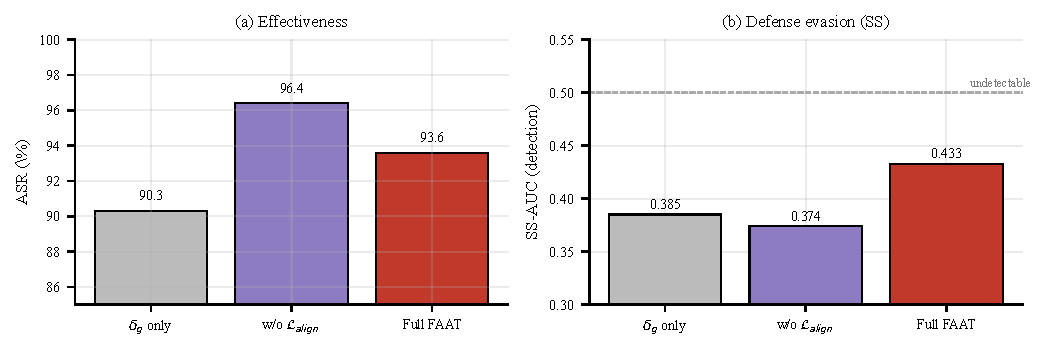
\includegraphics[width=\linewidth]{floats/figures/f6_ablation.pdf}
\caption{\textbf{Component ablation} (CIFAR-10, $\ell_2\!=\!1.5$). Removing
$\Lalign$ slightly raises ASR but \emph{lowers} defense evasion (SS-AUC moves
away from the undetectable $0.5$); $\Lalign$ is thus a stealth component rather
than an ASR component.}
\label{fig:ablation}
\end{figure}

\begin{figure}[t]
\centering
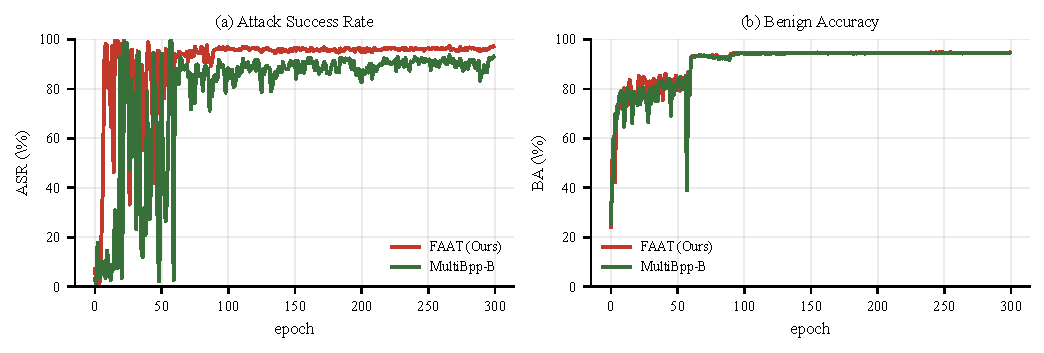
\includegraphics[width=\linewidth]{floats/figures/f7_convergence.pdf}
\caption{\textbf{Training dynamics} on CIFAR-10. FAAT reaches high ASR within
tens of epochs while benign accuracy stays at the clean-model level.}
\label{fig:conv}
\end{figure}


\paragraph{Role of each component.}
Table~\ref{tab:ablation} removes FAAT's components one at a time (CIFAR-10,
$\ell_2\!=\!1.5$). The bare global direction ($\dglobal$ only, i.e.\ a Narcissus
trigger) already reaches $90.3\%$ ASR---confirming $\dglobal$ supplies the bulk
of the backdoor signal. Adding $\dadapt$ and the full pipeline raises ASR to
$93.6\%$ \emph{and} improves stealth (SS-AUC $0.385\!\to\!0.433$). Removing
$\Lalign$ \emph{raises} ASR to $96.4\%$ but \emph{lowers} SS-AUC to $0.374$:
$\Lalign$ is therefore a \emph{stealth} component that trades a little ASR for
better defense evasion, exactly as designed (Sec.~\ref{sec:method}). SSIM is
stable ($0.95$) across variants.

\paragraph{Training dynamics.}
Figure~\ref{fig:conv} shows ASR and BA over $300$ epochs. FAAT crosses
$80\%$ ASR within the first $\sim$$16$ epochs and settles at $93.6\%$, while BA
stays at the clean-model level throughout---there is no benign-accuracy dip to
signal the attack.

\paragraph{Budget sensitivity.}
On CIFAR-10 the $\ell_2$ budget $\{0.9,1.2,1.5\}$ traces a smooth ASR--SSIM
frontier ($76.1 / 88.6 / 93.6\%$ at SSIM $0.98/0.97/0.95$, Fig.~\ref{fig:pareto});
$\sigma_{\asr}\!\le\!2.5$ across 3 seeds (see supp.).
Full per-dataset, per-seed numbers and the adaptive-generator ablation are in
the supplement.
